\documentclass[11pt,letterpaper]{report}
%%%%%%%%%%%%%%%%%%%%%%%
%% Page layout
\usepackage{graphics,graphicx,wrapfig}
\usepackage[letterpaper, margin=2.5 cm, headheight=4 cm, top= 6cm]{geometry}
\setlength{\parindent}{0pt}
\usepackage{parskip}
\setlength{\parskip}{0.5em}

\usepackage{fancyhdr}
\usepackage{bm}
\usepackage{upgreek}

\fancyhf{}
\fancyhead[L]{

\includegraphics[height=3 cm]{Figures/Brown_Letterhead/H_2c_Pos}
\\
}
%
\fancyhead[C]{
\parbox[b][3.5cm][t]{4cm}{
\begin{flushright}
Haneesh Kesari
\\
Assistant Professor
\\
of Engineering
\\
\end{flushright}
}
}
%
\fancyhead[R]{
\parbox[b][3.5cm][t]{6cm}{
\begin{flushleft}
School of Engineering
\\
Brown University
\\
184 Hope Street, B\&H 612
\\
Providence, RI 02912
\\
Phone: 401-863-1418
\\
Email: Haneesh\_Kesari@brown.edu
\\
\end{flushleft}
}
}

\fancypagestyle{plain}{
\fancyhf{} % remove everything
%
\renewcommand{\headrulewidth}{0pt} % remove lines as well
%
\renewcommand{\footrulewidth}{0pt}
%
\fancyfoot[R]{\thepage / \pageref{LastPage}}
}

%% Fonts
\usepackage{amssymb,amsfonts,amsmath,amsthm}
\usepackage[T1]{fontenc}
\usepackage{mathptmx}
\usepackage{cmbright}
\usepackage{bm}

\usepackage{sectsty}
\sectionfont{\fontsize{16}{16}\selectfont}

%% typesetting
\usepackage{tabto}
\usepackage{upgreek}

%% colors
\usepackage[dvipsnames]{xcolor}
\definecolor{DarkRed}{rgb}{0.62, 0.16, 0.09}

%% referencing
\usepackage{nameref}
\usepackage{lastpage}
\usepackage[biblabel]{cite}
\usepackage[english]{babel}
\usepackage{natbib}
\bibliographystyle{abbrvnat}
\setcitestyle{authoryear,open={(},close={)}} %Citation-related commands
\usepackage[colorlinks=true,urlcolor=DarkRed,linkcolor=DarkRed,citecolor=black]{hyperref}

%% enumerate
\usepackage{enumerate}
\usepackage{enumitem}

%% floats
\usepackage{float}
\usepackage[font=footnotesize, labelfont={bf},labelsep=period]{caption}
\usepackage{booktabs}
\usepackage{threeparttable}

%% custom commands
\usepackage[scr=boondoxo]{mathalfa}
\newcommand{\loc}{\textit{LoC}}

\newcommand{\norm}[1]{\ensuremath \lVert #1 \rVert}

\newcommand{\ex}{{\bm{\hat{e}}}_1}
\newcommand{\ey}{{\bm{\hat{e}}}_2}
\newcommand{\ez}{{\bm{\hat{e}}}_3}
\newcommand{\ei}{{\bm{\hat{e}}}_i}
\newcommand{\ej}{{\bm{\hat{e}}}_j}
\newcommand{\er}{{\bm{\hat{e}}}_r}
\newcommand{\et}{{\bm{\hat{e}}}_\theta}
\newcommand{\ep}{{\bm{\hat{e}}}_\phi}

\usepackage{xspace}
\newcommand{\TA}{\textit{Ta.\@}\xspace}
\newcommand{\EA}{\textit{Ea.\@}\xspace}

%% checklist
\usepackage{enumitem,amssymb}
\newlist{todolist}{itemize}{2}
\setlist[todolist]{label=$\square$}
\usepackage{pifont}
\newcommand{\cmark}{\ding{51}}%
\newcommand{\xmark}{\ding{55}}%
\newcommand{\done}{\rlap{$\square$}{\raisebox{2pt}{\large\hspace{1pt}\cmark}}%
\hspace{-2.5pt}}
\newcommand{\wontfix}{\rlap{$\square$}{\large\hspace{1pt}\xmark}}


\renewcommand{\u}[1]{\boldsymbol{#1}}
\renewcommand{\t}[1]{\tilde{#1}}
\newcommand{\m}[1]{\mathbb{#1}}
\renewcommand{\c}[1]{\mathcal{#1}}
\newcommand{\lsc}[2][\mathscr{l}]{{}^{ #1 }\! #2}
\newcommand{\lscH}[1]{\lsc[H]{#1}}
\newcommand{\dsf}[1]{\Delta\boldsymbol{\sf #1}}
\newcommand{\tpsb}[1]{\left. #1 \right.^{\sf T}}
\newcommand{\tps}[1]{\left( #1 \right)^{\sf T}}
\newcommand{\usf}[1]{\boldsymbol{\sf #1}}
\newcommand{\busf}[1]{\bar{\usf{ #1}}}
\newcommand{\tu}[1]{\tilde{\u{ #1}}}
\newcommand{\tusf}[1]{\tilde{\usf{ #1}}}
\newcommand{\btusf}[1]{\bar{\tusf{ #1}}}
\newcommand{\pr}[1]{\left( #1 \right)}
\newcommand{\physe}{\hat{\mathbscr{e}}} %


\begin{document}

\newpage
\setcounter{page}{1}
%%%%%%%%%%%%%%%%%%%%%%%%%%%%%%%%%%%%%%%%%%%%%%%%%%%%%%
%%%%%%%%%%%%%%%%%%%%%%%%%%%%%%%%%%%%%%%%%%%%%%%%%%%%%%
%%%%%%%%%%%%%%%%%%%%%%%%%%%%%%%%%%%%%%%%%%%%%%%%%%%%%%
\thispagestyle{fancy}
\phantom{x}
\vspace{4em}
% \textbf{Author response letter to Reviewers}

Regarding: Point-by-point response to issues raised by referees  (manuscript JMBBM-D-21-00364).
%hk done

\vspace{3em}
Dear Editors and Reviewers,
%hk done
\vspace{1em}

We thank you for your very valuable feedback. In response to your feedback, we have made the revisions listed in the section \textit{List Of Changes} (\textit{LoC}), which can be found on  page \pageref{LoCpage} of this response letter. We  provide a point-by-point response to the Reviewers' comments in the following pages. Our responses to Reviewer \#1's and Reviewer \#2's comments can be found on pages \pageref{rev1} and \pageref{rev2}, respectively, of this response letter. Through these changes and our responses to your comments, we hope that we have addressed all of your concerns.

We thank you for your consideration of our revised manuscript.

\vspace{2em}
Sincerely,

Wenqiang Fang, Sayaka Kochiyama, and Haneesh Kesari

%%%%%%%%%%%%%%%%%%%%%%%%%%%%%%%%%%%%%%%%%%%%%%%%%%%%%%
%%%%%%%%%%%%%%%%%%%%%%%%%%%%%%%%%%%%%%%%%%%%%%%%%%%%%%
%%%%%%%%%%%%%%%%%%%%%%%%%%%%%%%%%%%%%%%%%%%%%%%%%%%%%%
\clearpage
\pagestyle{plain}
\newgeometry{margin=2.5 cm}
%%%%%%%%%%%%%%%%%%%%%%%%%%%%%%%%%%%%%%%%%%%%%%%%%%%%%%
\section*{List of Changes}
\label{LoCpage}
The following changes  appear in red in the revised version of the manuscript.
% {\bf Changes in response to Reviewer criticisms}

% \begin{enumerate}[label=\textit{Mc.\arabic*}]
% %
% \item \label{a1} In response to Reviewer \#1's comment (listed as comment \ref{r1c3} of this letter) regarding the existing frameworks for estimating head accelerations, we have modified the third paragraph in page 4. We added the work of Genin \textit{et al.}~\cite{genin1997} as a reference.
% %
% \item \label{a2} In response to Reviewer \#1's comment (listed as comment \ref{r1c4} of this letter) regarding the existing frameworks for estimating head accelerations, we have modified the third paragraph in page 4. We added the works of Madgwick \textit{et al.}~\cite{madgwick2013} and Naunheim \textit{et al.}~\cite{naunheim2003} as references.
% \end{enumerate}

\clearpage
%%%%%%%%%%%%%%%%%%%%%%%%%%%%%%%%%%%%%%%%%%%%%%%%%%%%%%
\section*{Response to Reviewer \#1's comments}
\label{rev1}

\begin{enumerate}[label=\textit{1.\arabic*},wide, labelwidth=!, labelindent=0pt]

\item \label{r1c1} {\bf ``The authors have presented a good piece of work, through which they are able to explain the sawtooth patterns observed in the force-displacement curves. This is done by allowing for slippage at the test supports and paying attention to the coefficient of friction.''}

% We thank the Reviewer for their consideration of our manuscript.


We thank the Reviewer for their very generous comments regarding our manuscript.

\newpage
\item \label{r1c2} {\bf `` A few minor comments to help clarify and strengthen the work: a) In the SS experiments, how it is ascertained that the boundary conditions correspond to the simply supported conditions.''}

% We thank the reviewer for the comments on helping clarify and strengthen the work.

We thank the reviewer for their feedback on how to clarify and strengthen our arguments.


We use the phrase ``simply supported'' to connote that there were no bending moments acting at the spicule's supports. We assume that there are no bending moments acting at the spicule's supports due to the following three reasons.

1. The experiments that we refer to as simply supported were set-up by simply placing the spicules on the mechanical testing stage, across the trench; and not using glue or any other means to render the spicules immobile on the stage (e.g., see Fig.~\ref{fig:photos} (A) and (C)). Partly due to this reason, the spicules experienced no adhesive interaction with the stage. This was  quite evident to us from the  tremendous difficulty we faced in getting the spicules to their proper positions across the trench. (A proper position was one in which
the spicules lay symmetrically across the trench, and their entire length lay in the focal plane of the experiment's optical microscope.)  Since the spicules had no adhesive interaction with the stage, no bending moments could act on them at their supports (trench edges).

2. We collected optical microscopy images of the spicule's deformed configurations during the experiments. The experiments that we modeled were originally reported in~\citet{monn2017enhanced}. Additional experiments to support the hypothesis that we presented in the current manuscript were presented in~\citet{kochiyama2021sawtooth}. The optical images of the spicule's deformed configurations can be found in  Fig. 3 of~\citet{monn2017enhanced} and Fig. 5 of~\citet{kochiyama2021sawtooth}. For the Reviewer's convenience, we also present some of those images in Fig.~\ref{fig:photos}. In all those images it can be observed that the
sections of the spicule that lie outside the trench (i.e., towards the left and right  of the trench) always have a straight shape. (In Fig.~\ref{fig:photos} (B) and (D), the spicule sections lying outside the trench are marked using  white dashed ellipses.) As per elementary beam theories, these straight shapes are only possible if there are no bending moments acting at the supports.



% \begin{figure}[H]
% \centering
% 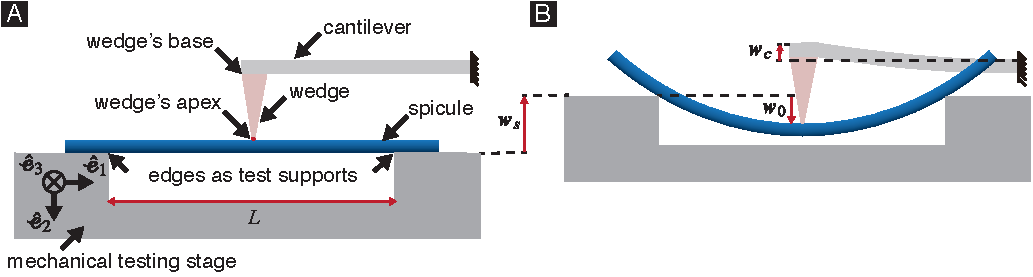
\includegraphics[width = 1.0\textwidth]{Figures/SSsetup_V4.pdf}
% \caption{An illustration of the simply-supported setup (Figure 5 of the submitted manuscript).}
% \label{fig:SSsetup}
% \end{figure}

\begin{figure}[H]
\centering
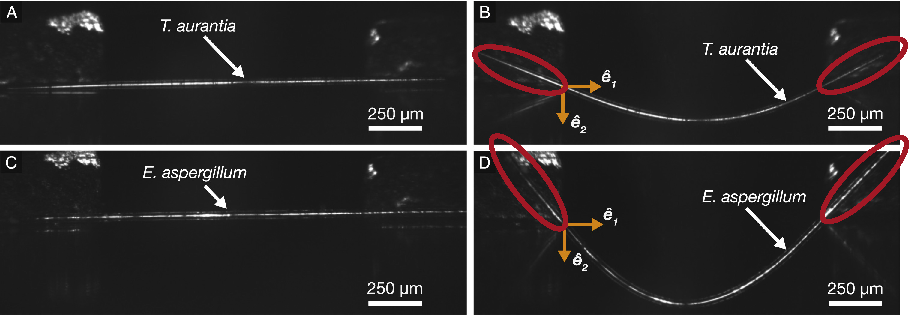
\includegraphics[width = 1.0\textwidth]{Figures/Straight.pdf}
\caption{(A) and (B) (resp. (C) and (D)) show the undeformed configuration and deformed configuration just before failure of a representative \textit{Tethya aurantia} (resp. \textit{Euplectella aspergillum}) spicule (adapted from Fig. 3 of~\citet{monn2017enhanced}). In (B) and (D) the spicule segments lying outside the trench  are marked using white ellipses.}
\label{fig:photos}
\end{figure}


3. On assuming simply-supported boundary conditions, the predictions from the  elastica  theory for the deformed shapes of the spicules match remarkably well with the shapes' measurements  from the optical microscopy images (see Fig.~\ref{fig:EBMatch}).  We employed no  fitting parameters when comparing the predictions for the deformed shapes with their optical microscopy measurements. The lengths and diameters were measured independently from optical and scanning electron microscopy imaging, and the Young's modulus was measured independently from the force-deflection measurements.

\begin{figure}[H]
\centering
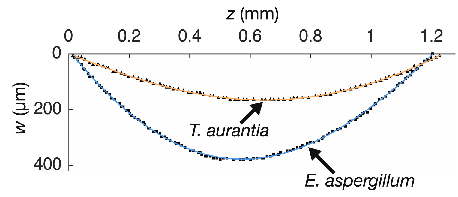
\includegraphics[width = 0.6\textwidth]{Figures/EBMatch.pdf}
\caption{
Comparison of the predictions from the  elastica  theory for the deformed shapes of the spicules  with the shapes' measurements  from  optical microscopy images.
 The black triangles (resp. squares) mark the measured  positions of the material points from the mid-axis of the \textit{Tethya aurantia} (resp. \textit{Euplectella aspergillum}) spicule shown in Fig.~\ref{fig:photos} (B) (resp. (D)). The orange (resp. blue) curves correspond to the deformed shapes predicted by the elastica theory. (adapted from Fig. 4(D) of~\citet{monn2017enhanced}).}
\label{fig:EBMatch}
\end{figure}

\newpage
\item \label{r1c3} {\bf ``b) The experiments all appear to be conducted for a static loading and this needs to be pointed out explicitly, in particular, when using friction in the model. The time scales over which the loading could be critical if dynamic friction is involved. Can any relevant details be provided in the paper?
''}

We thank the reviewer for pointing out this lapse on our part. In order to rectify this lapse  we  have made the following changes.


(i) In \S \textcolor{red}{xx} of the revised manuscript,  we now explicitly state that, in our model, each of the configurations for which we derive quantitative predictions are taken to be in static equilibrium.

(ii) We now provide details about the stage's motion and the time scales involved in the experiment in the revised version of the manuscript. These newly added details appear in red in the third paragraph of $\S$3 of the revised manuscript. We repeat those details below for the Reviewer's convenience.

Note that in the below quote MTS stands for Mechanical Testing Stage.

\textit{The loading phase of the tests were conducted by moving the MTS in
 the~$-\physe_2$ direction at an average velocity of ~$\approx 1~\mu\rm m/sec$. The MTS was driven by a DC servo motor, whose motion was controlled through a PID algorithm. The stage was moved in  $2~\mu \rm m$ increments. During the increment, the stage's velocity was maintained between ~$50$ and $200~\mu \rm m/sec$. Thus, each  stage increment took anywhere between $10$ and $40~\rm{ms}$. After each increment, the stage was held motionless so that there was a $2100~\rm{ms}$ time interval  between the starting points of any two consecutive increments. Each data point that we report was calculated using the  average value of the sensor readings collected over the last $100~\rm{ms}$ of one of those time intervals.}


 % It is true as the reviewer points that each   configuration that theory model is a static configuration.

 % , the time history of the system through which can the sytems find in that configuration cannot be ignored. so as not suprress any future interpretation of our experiments using dynamic frictional effects, or aging effects related to friction.



 % as the reviewer as so astutrely noted depending on the  time-scales the dynamic friction could be important.

\newpage
\item \label{r1c4} {\bf ``
c) With regard to the elastica theory, an extension would be the rod theory, which would be needed for a three-dimensional setting; see Antman, S. S., Problems in Nonlinear Elasticity, Springer.''}

% Although we have introduced our mathematical notions and definitions in a general three-dimensional context, we clearly stated that our modelling the spicule's deformation is two dimensional in the last paragraph in page 6 of the manuscript:
% ``Considering the geometry in the SS experiments (e.g., see Figure~2), in our model we take that the spicule's displacements to be two dimensional in nature.''

% We were looking for an extension of Euler-Bernoulli (EB) theory to the regime of large displacements and rotations in our study. We believe Euler's elastica theory is sufficient and mathematically tractable.
% The rod theory is a more general extension of elastica theory, which accounts for not only flexure, but also extension and shear.
% In our experimental setup, the effects of extension and shear do not play an important role in the deformation of the spicules. Thus we believe that it is reasonable to ignore the effects of extension and shear in the model. Therefore, we modeled the spicules' deformation using Euler's elastica theory.

We thank the Reviewer for bringing up the rod theory and encouraging us to expand our model to the 3D context. We are very interested in that type of a generalization, and thank the Reviewer for their encouragement and guidance.

% In fact, to account for the effects of the multi-layer architecture on the large deflection of \textit{E. aspergillum} spicules, we have proposed a homogenized finite shear deformable beam theory~\cite{FangShearBeam}, in which we developed a shear deformable beam theory in a systematic way by following the general three-dimensional continuum theory and employing the Hellinger-Reissner variational principle. Neither the shear deformable beam theory or the rod theory by Antman comes with analytical solutions. When dealing with complicated beam deformation, such as buckling and looping formation, numerical instabilities are inevitable. Therefore, in order to get neat analytical solutions, we modeled the spicules' deformation using Euler's elastica theory in the submitted manuscript. We thank the reviewer again for providing such great insights and we will explore further in that direction in the future.



% \end{enumerate}


\clearpage

%%%%%%%%%%%%%%%%%%%%%%%%%%%%%%%%%%%%%%%%%%%%%%%%%%%%%%
\section*{Response to Reviewer \#2's comments}
\label{rev2}

\begin{enumerate}[label=\textit{2.\arabic*},wide, labelindent=0pt]

\item \label{r2c1}{\bf ``The authors report on the three-point bending tests of marine sponge fibers and the possible mechanism for the sawtooth-pattern during the bending tests. They argued that the sawtooth-pattern is originated from the stick-slip motion on the supporting substance and eliminated the Cook-Gordon mechanism.
While Cook-Gordon mechanism is valid during the fracture of the materials, I am curious whether the experiment here caused the fracture of the spicule?
If not, then the bending of spicule may remain in the "elastic deformation" and the stick-slip should be caused by the friction on the supporting layer, as stated by the authors. Then the initial argument is meaningless.
If yes, how is the fractured surface looks like? Will the propagation of cracks have any correlation to the sawtooth-pattern? ''}



All  sawtooth patterns that we attempt to explain in our manuscript are from experiments in which the spicules were loaded until failure. Some of the spicule
 fractured surfaces are shown in Fig.~\ref{fig:Surfaces}.

\begin{figure}[H]
\centering
\includegraphics[width = 1.\textwidth]{Figures/Surfaces.pdf}
\caption{Force-displacement curves and optical images of the fractured surfaces for (A and B) \textit{Monorhaphis chuni} anchor spicules, (C and D) \textit{Rosella racovitzae} spicules (adapted from Fig. 4 of~\citet{kochiyama2021sawtooth}), and (E and G) \textit{Euplectella aspergillum} (\textit{Ea.}) anchor spicules (adapted from Fig. 3 of~\citet{monn2017enhanced}).
}
\label{fig:Surfaces}
\end{figure}

In Fig.~\ref{fig:Surfaces}, the experiments on \textit{Ea.} spicules were performed by us, while the experiments on \textit{M. chuni} and \textit{R. racovitzae} are taken from literature.


Regarding the Reviewer's question of "Will the propagation of cracks have any correlation to the sawtooth-pattern?" we have not measured the evolution of the crack(s) with loading in our experiments. (Only the final fracture surfaces, as those shown in Fig.~\ref{fig:Surfaces}, are available.) Neither is such information available for the experiments on \textit{M. chuni} and \textit{R. racovitzae}. Measurement of the crack(s) evolution in spicules during loading is quite a challenging task due to the length scales involved (the \textit{Ea.} spicules are typically 50 micrometer in diameter), and the fact that the crack(s) surface(s) can be 3D and/or multiply connected in nature. Since no data is available on how the crack(s) evolve during the loading process, we cannot answer whether or not the "propagation of cracks have any correlation to the sawtooth-pattern." We can only comment that if such a correlation is indeed observed then that would be evidence against our hypothesis, and if no such correlation is found then that would further strengthen our hypothesis.

In the work of~\citet{clegg1990simple}, a correlation was found between the evolution of the crack(s) and the drops in the force-deflection curve. The correlation of the evolution of the crack(s) with the force-deflection curve in the work of Clegg et al. is a reflection of the operation of the Cook-Gordon mechanism, whereby the interfaces repeatedly arrest crack growth, leading to a toughening effect. However, recent experiments and large scale fracture simulations~\cite{monn2020lamellar} have revealed that the spicules are not significantly tougher compared to the biogenic silica that composes them, and that the Cook-Gordon mechanism is suppressed in them due to the curved nature of the interfaces.

% However, as the crack may grow inside the spicules, optical micrographs can not provide such evidence. Sophisticated experimental design involving electric circuit may be effective for the purpose of monitoring crack propagation.
% Since we have difficulty monitoring the crack propagation during our tests, we cannot conclude whether the propagation of cracks have any correlation to the sawtooth pattern solely from the final fractured surfaces of the spicules after the tests.


\newpage
\item \label{r2c2}{\bf ``The labelling of figures is chaos! The language should be polished, it is quite spoken language.''}
\end{enumerate}

In response to the reviewer's above comments, we have made the following two changes.

(i) Regarding the comment that the labeling is unclear, we believe that what led to this comment was the wrong figures being referred to at some locations in the text. For example, in the fifth and sixth paragraphs of $\S$1 in the original submission, Figure $1$ was incorrectly referred to instead of Figure $3$. We have corrected these incorrect references in the revised version of the manuscript.

(ii) Regarding the Reviewer's concern about the language appearing "spoken," we have tried our utmost to address this comment by changing the text at several locations in the revised version of the manuscript.


\end{enumerate}

\clearpage

%%%%%%%%%%%%%%%%%%%%%%%%%%%%%%%%%%%%%%%%%%%%%%%%%%%%%%
\bibliographystyle{apalike}
\bibliography{refs}

\end{document}

WF:
1. LoC.
2. Things marked XX.


SK :

1. Spoken writing in the text.
2. Read the entire response letter after WF says he is done with it.
